In the period M25-M30, the monitoring component was developed and integrated within the scope of WP8.\\
The monitoring framework is responsible for the monitoring of the overall SmartSociety platform and components. It acts as a central collection point for any information which is considered important to ensure the proper functioning of the platform. Target users of the monitoring components are system administrators who need to check the status of the system and the liveness of the services. 

The monitoring framework allows to:
\begin{itemize}
\item Dynamically collect diverse information relevant for monitoring the proper functioning of the platform and its performance. Such information is permanently stored in a non-relational database and available at any time for inspecting specific platform behaviors.
\item Visualize such information in real-time by means of interactive dashboards, or query the collected data via dedicated APIs. %In particular, through the Monitoring framework it is possible to create and configure specific visualizations starting from the data that has been collected. There can be multiple visualizations, each one geared towards a specific platform KPI or informative visualization.
\end{itemize} 

%first, it allows to permanently store the data that is collected from the various COMPOSE components. The information can then be explored over time in order to either analyse the performance of platform components, or identify the causes of a specific malfunctioning. 
%Second, it allows to visualize both real-time, as well historical data. In particular, through the Monitoring dashboard it is possible to create and configure specific visualizations starting from the data that is collected. There can be multiple visualizations, each one geared towards a specific platform KPI or information.
%The COMPOSE platform administrator is expected to be the key utilizer of the Monitoring Dashboard. The current implementation does not support different visualizations based on user role.

The high-level architecture of the monitoring component is represented in~\ref{fig:monitoringArch}.
%Monitoring Dashboard is based on the following architecture and components:


\begin{figure}[!hbt]
\centering
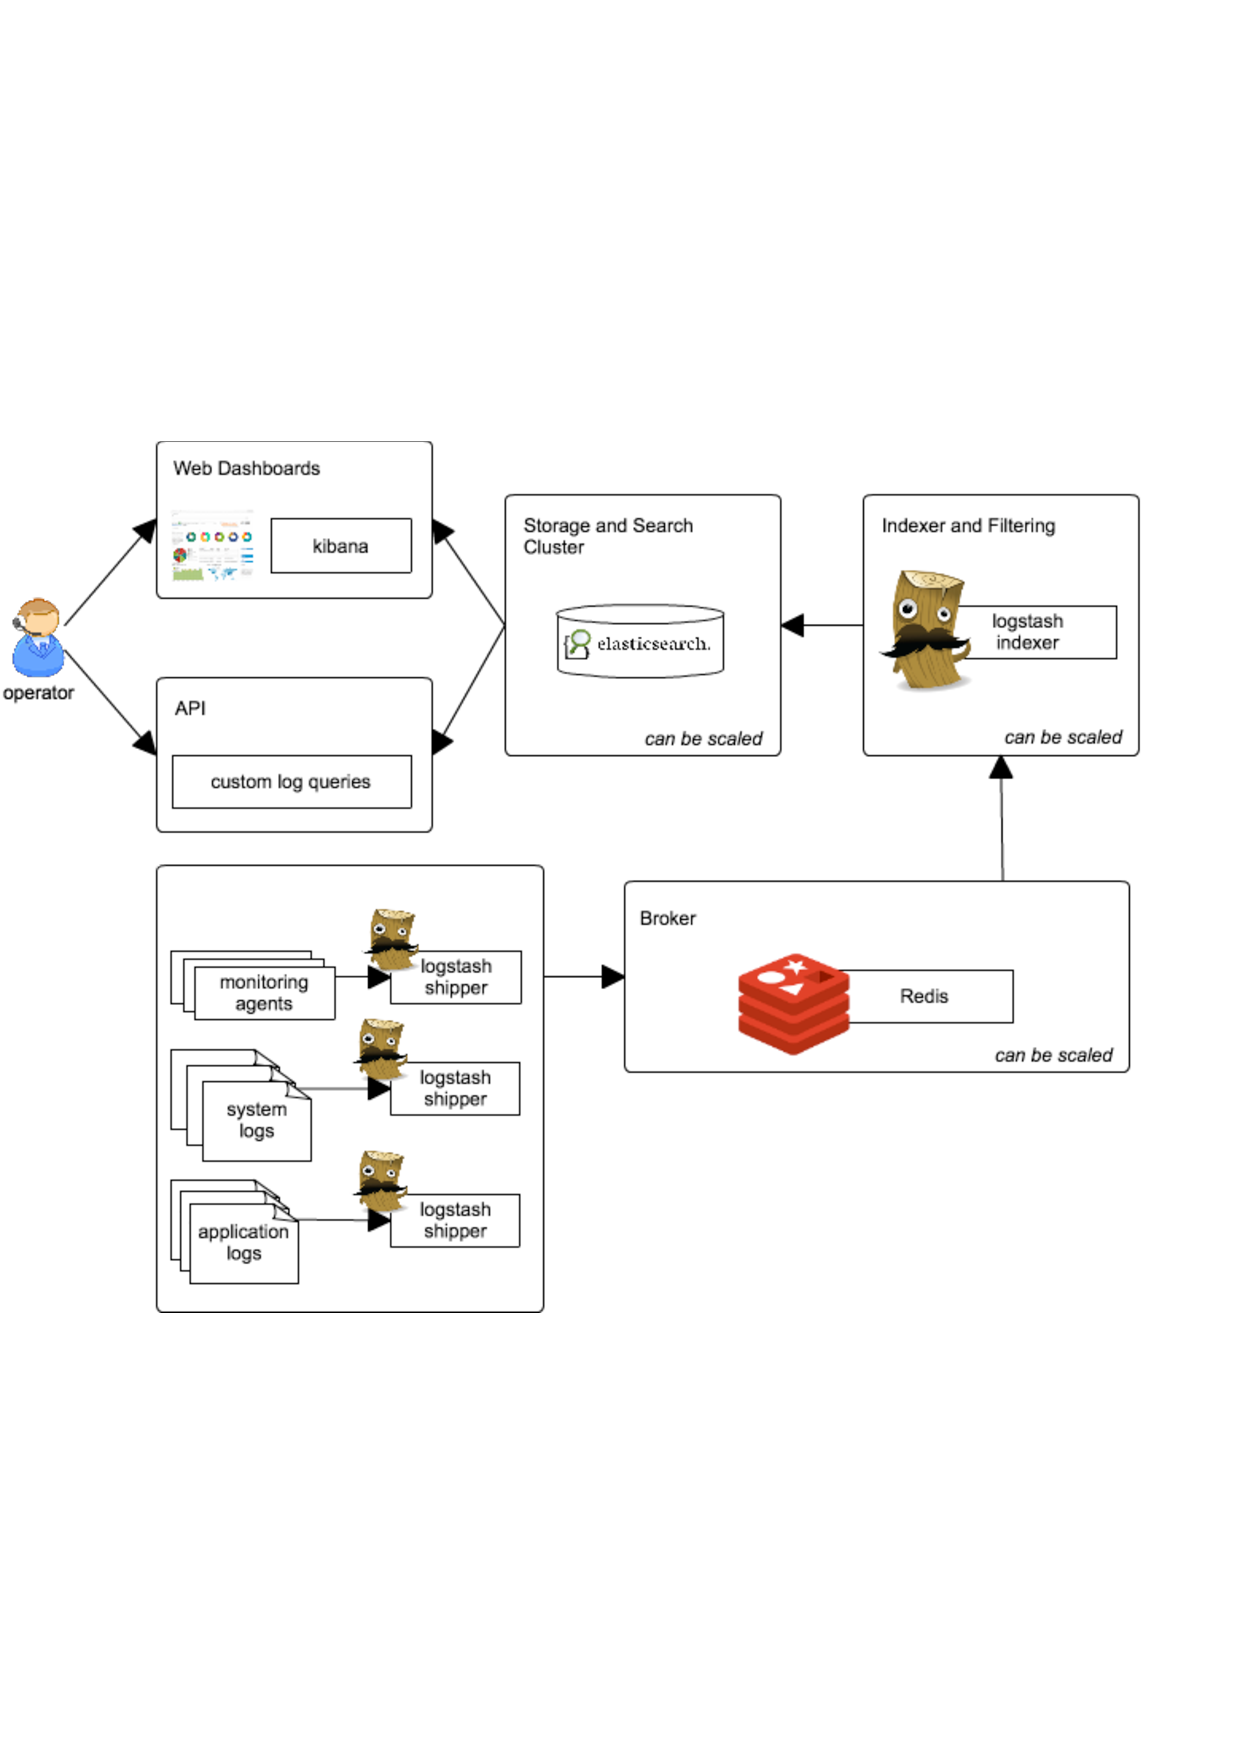
\includegraphics[width=0.8\textwidth]{figs/monitoring.pdf}
\caption{Monitoring framework architecture.}
\label{fig:monitoringArch}
\end{figure}

The monitoring framework is based on Logstash\footnote{{\tt http://logstash.net/}}, an open-source tool for managing events and logs. Logstash can be used to collect logs, parse them, and store them for later use (e.g., search and visualization). %Speaking of searching, Logstash comes with a web interface for searching and drilling into all of the logs collected over time.
It is possible to define what information shall be permanently stored and processed by the monitoring framework. In particular, it is possible to integrate:
\begin{itemize}
\item System logs: these logs correspond to logs, which are generated by the various system components such as, e.g., web servers, application servers. 
\item Application logs: specific logs that are produced by applications, and require a constant integration for debugging and monitoring purposes.
\item Monitoring information: any agent that can be configured to deliver data to the Logstash infrastructure.
\end{itemize}

In all three cases, a Logstash shipper is used to connect the specific source of data to Logstash. Specific shippers already exists for some widely used system components such as, e.g., web servers, databases, etc., while custom shippers can be created for specific cases. In the case of SmartSociety, we created a dedicated shipper to collect the events produced by the various platform components.\\
The following component is a Redis Broker. This is an optional component that can be used in order to scale the system to large volumes of events and data. Based on Redis, data is indexed in order to prepare it for optimal searching and querying. Once the data is indexed, it is stored in an ElasticSearch cluster for storage and search. 
Starting from the data stored in ElasticSearch, it is possible to build queries on scale to explore the collected data. We decided to use Kibana\footnote{{\tt https://www.elastic.co/products/kibana}} as the tool to create and visualize queries on the collected data. Kibana is fully integrated with ElasticSearch, and allows to easily explore and analyze large volumes of data. A sample visualization is shown in~\ref{fig:kibana}.  The metrics and specific charts can be configured dynamically by the administrator of the platform.

In addition, ElasticSearch provides APIs for querying and extracting the data stored in the platform. This can be helpful in the case aggregated views such as, e.g., monthly reports, are needed.

\begin{figure}[!hbt]
\centering
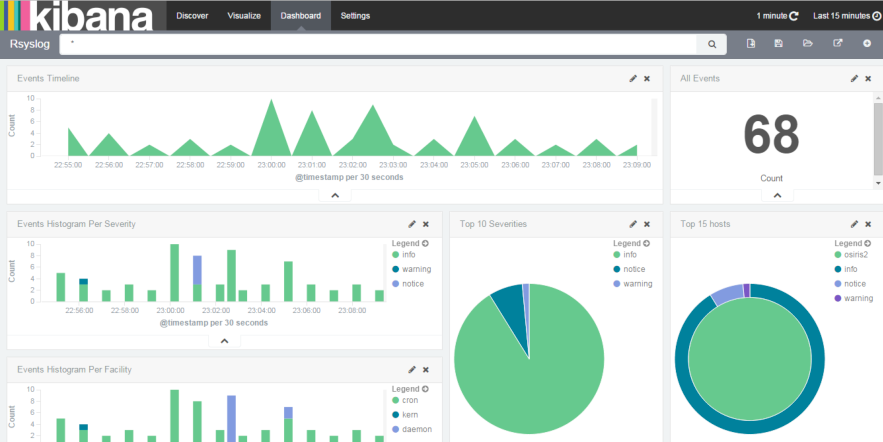
\includegraphics[width=0.8\textwidth]{figs/kibana.pdf}
\caption{Example of the monitoring framework web interface.}
\label{fig:kibana}
\end{figure}
